% ----------------------------------------------------------
% 7. Diagrama de Classes
% ----------------------------------------------------------
\chapter{Diagrama de Classes}
\label{cap:diagrama-classes}

Nesta seção é apresentado o Diagrama de Classes do sistema de gestão da Commit Júnior, elaborado sob a ótica da modelagem conceitual e lógica orientada a objetos[cite: 6, 20]. O diagrama foi modelado com o objetivo de refletir fielmente as entidades, relacionamentos, atributos e operações identificados ao longo do levantamento de requisitos, mantendo total rastreabilidade com o Minimundo, o Diagrama de Casos de Uso (DCU) e os protótipos de interface desenvolvidos[cite: 6, 20].

\begin{figure}[!htbp]
    \centering
    \caption[Diagrama de Classes do Sistema da Commit Júnior]{Diagrama de Classes do Sistema de Gestão de Membros da Commit Júnior}
    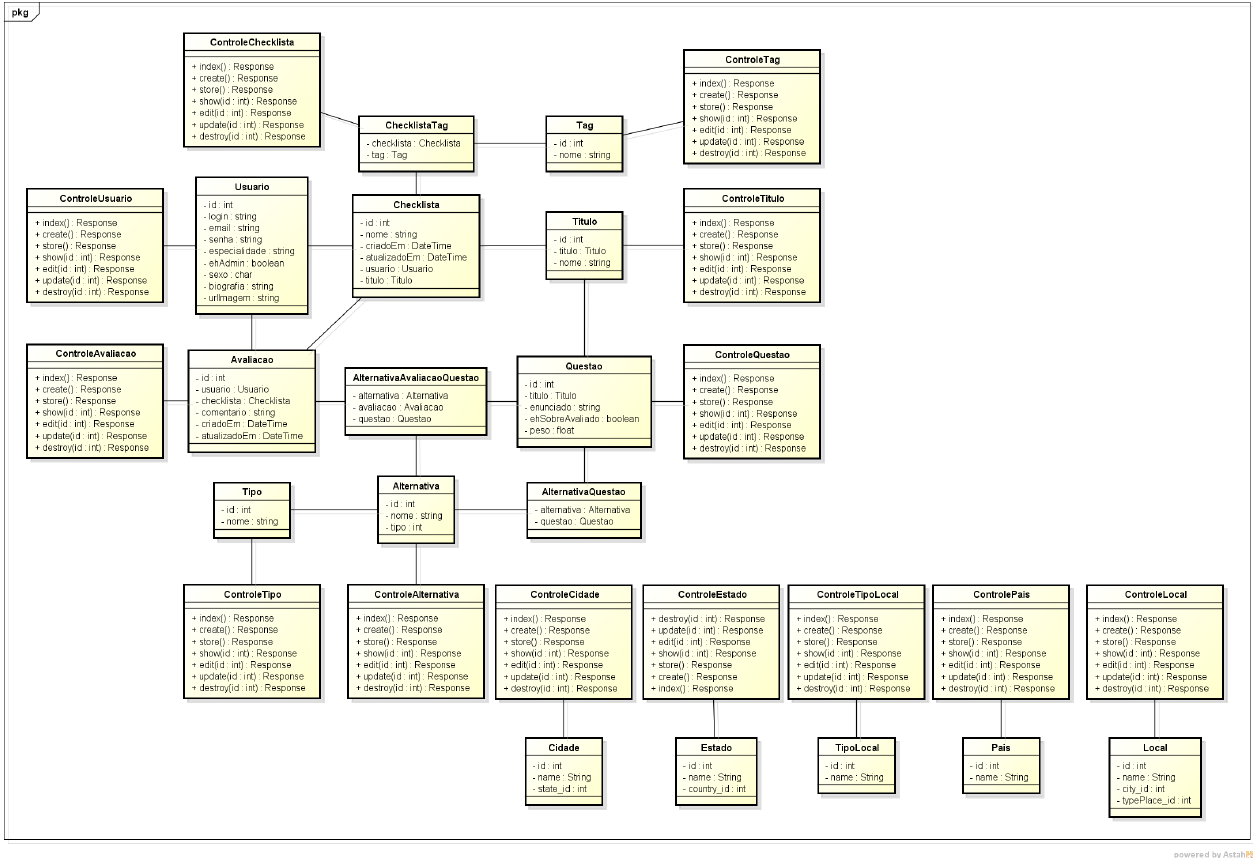
\includegraphics[width=0.98\textwidth,keepaspectratio]{exemplo-diagrama-classes.png}
    \label{fig:diagrama-classes}
\end{figure}

\section*{Descrição das Classes e Relacionamentos}

Para assegurar a completude e clareza da arquitetura de dados e domínio, as principais classes do modelo são descritas a seguir[cite: 20]:

\begin{itemize}
    \item \textbf{Membro:} Classe central do domínio que encapsula as informações cadastrais civis, acadêmicas e funcionais de cada integrante (como matrícula, CPF, RG, nome completo, curso, e-mail institucional, perfil de GitHub, status no sistema e data de ingresso)[cite: 1, 2, 4]. Implementa os métodos de controle de ciclo de vida e inativação lógica requeridos pelas regras de negócio[cite: 20].
    
    \item \textbf{Usuario / PerfilAcesso:} Responsável pelos mecanismos de autenticação, armazenamento seguro de credenciais (hash de senha) e autorização baseada em papéis (RBAC), segregando os privilégios entre Administrador, Jurídico, Líder de Área e Membro.
    
    \item \textbf{Cargo / Funcao e RegraHoras:} Entidades que parametrizam a estrutura organizacional (Diretoria, Squad) e definem a taxa de horas de extensão atribuída a cada atividade desempenhada por intervalo de vigência[cite: 1, 4].
    
    \item \textbf{HistoricoCargo / Extensao:} Associação temporal entre o membro e as funções desempenhadas, permitindo computar com precisão o tempo de permanência na empresa e o acumulado de horas de extensão para fins acadêmicos[cite: 1].
    
    \item \textbf{EnvioHorasCoordenacao:} Registra o lote de horas consolidadas que é gerado e despachado formalmente via correio eletrônico institucional (protocolo SMTP) ao professor orientador da Commit Júnior para homologação e lançamento no SIGAA[cite: 1].
    
    \item \textbf{TermoJuridico:} Gerencia os contratos obrigatórios de voluntariado, termos de rescisão/desligamento e certificados[cite: 2]. Mantém os códigos de autenticidade, links e o estado das assinaturas digitais intermediadas pelo serviço externo[cite: 2].
    
    \item \textbf{OcorrenciaPontuacao e Contestacao:} Modela o controle disciplinar da empresa júnior[cite: 3]. Registra infrações, saldo de pontos, prazos calculados de expiração e incidência de agravantes de reincidência, permitindo o acoplamento de justificativas formais abertas pelos membros[cite: 3].
    
    \item \textbf{Aviso:} Entidade responsável pelas publicações do mural de informes, admitindo segmentação geral institucional ou restrição por diretoria específica.
    
    \item \textbf{Compromisso / Evento:} Modela os compromissos corporativos plenários (Reuniões Gerais, imersões) e as reuniões individuais bilaterais (1-on-1), com validação de choques de horário entre os participantes.
\end{itemize}

\section*{Integração com Sistemas Externos}

Conforme especificado no Minimundo e nas regras de negócio, determinados dados e eventos interagem com plataformas e atores externos[cite: 20]:

\begin{itemize}
    \item \textbf{Autentique (Serviço de Assinatura Eletrônica):} Plataforma externa responsável pelo fluxo de coleta de assinaturas digitais nos termos contratuais e certificados[cite: 2]. O sistema armazena apenas a referência do documento, código de autenticação e status de retorno[cite: 2].
    
    \item \textbf{Servidor SMTP Institucional:} Subsistema de mensageria responsável pela entrega dos relatórios formais de extensão e comunicados de desligamento por e-mail[cite: 6].
    
    \item \textbf{SIGAA (CEFET-MG):} Sistema acadêmico institucional para o qual as horas de extensão aprovadas são transcritas pelo professor orientador da Commit Júnior[cite: 1]. O sistema proposto não realiza inserções diretas no banco de dados do SIGAA, atuando na geração dos demonstrativos auditáveis que subsidiam esse lançamento externo[cite: 1].
\end{itemize}

\clearpage